\documentclass[tikz,border=2pt]{standalone}
\begin{document}
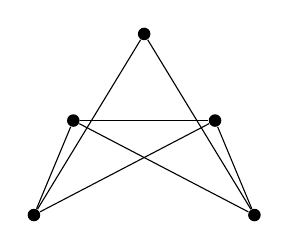
\begin{tikzpicture}[vertex/.style={circle,fill,inner sep=1.6pt}]
    \node[vertex] (b) at (0,2)       {};
    \node[vertex] (d) at (-0.9,0.9)  {};
    \node[vertex] (e) at (0.9,0.9)   {};
    \node[vertex] (a) at (-1.4,-0.3) {};
    \node[vertex] (c) at (1.4,-0.3)  {};

    \draw (d) -- (e);
    \draw (d) -- (a);
    \draw (d) -- (c);
    \draw (e) -- (a);
    \draw (e) -- (c);
    \draw (b) -- (a);
    \draw (b) -- (c);
\end{tikzpicture}
\end{document}
